\documentclass[journal,12pt,twocolumn]{IEEEtran}

\usepackage{setspace}
\usepackage{gensymb}
\singlespacing
\usepackage[cmex10]{amsmath}
\usepackage{amssymb}
\usepackage{xurl}

\usepackage{amsthm}
\usepackage{comment}
\usepackage{mathrsfs}
\usepackage{txfonts}
\usepackage{stfloats}
\usepackage{bm}
\usepackage{cite}
\usepackage{cases}
\usepackage{subfig}

\usepackage{longtable}
\usepackage{multirow}

\usepackage{enumitem}
\usepackage{mathtools}
\usepackage{steinmetz}
\usepackage{tikz}
\usepackage{circuitikz}
\usepackage{verbatim}
\usepackage{tfrupee}
\usepackage[breaklinks=true]{hyperref}
\usepackage{graphicx}
\usepackage{tkz-euclide}

\usetikzlibrary{calc,math}
\usepackage{listings}
    \usepackage{color}                                            %%
    \usepackage{array}                                            %%
    \usepackage{longtable}                                        %%
    \usepackage{calc}                                             %%
    \usepackage{multirow}                                         %%
    \usepackage{hhline}                                           %%
    \usepackage{ifthen}                                           %%
    \usepackage{lscape}     
\usepackage{multicol}
\usepackage{chngcntr}

\DeclareMathOperator*{\Res}{Res}

\renewcommand\thesection{\arabic{section}}
\renewcommand\thesubsection{\thesection.\arabic{subsection}}
\renewcommand\thesubsubsection{\thesubsection.\arabic{subsubsection}}

\renewcommand\thesectiondis{\arabic{section}}
\renewcommand\thesubsectiondis{\thesectiondis.\arabic{subsection}}
\renewcommand\thesubsubsectiondis{\thesubsectiondis.\arabic{subsubsection}}


\hyphenation{op-tical net-works semi-conduc-tor}
\def\inputGnumericTable{}                                 %%

\lstset{
%language=C,
frame=single, 
breaklines=true,
columns=fullflexible
}
\begin{document}


\newtheorem{theorem}{Theorem}[section]
\newtheorem{problem}{Problem}
\newtheorem{proposition}{Proposition}[section]
\newtheorem{lemma}{Lemma}[section]
\newtheorem{corollary}[theorem]{Corollary}
\newtheorem{example}{Example}[section]
\newtheorem{definition}[problem]{Definition}

\newcommand{\BEQA}{\begin{eqnarray}}
\newcommand{\EEQA}{\end{eqnarray}}
\newcommand{\define}{\stackrel{\triangle}{=}}
\bibliographystyle{IEEEtran}
\raggedbottom
\setlength{\parindent}{0pt}
\providecommand{\mbf}{\mathbf}
\providecommand{\pr}[1]{\ensuremath{\Pr\left(#1\right)}}
\providecommand{\qfunc}[1]{\ensuremath{Q\left(#1\right)}}
\providecommand{\sbrak}[1]{\ensuremath{{}\left[#1\right]}}
\providecommand{\lsbrak}[1]{\ensuremath{{}\left[#1\right.}}
\providecommand{\rsbrak}[1]{\ensuremath{{}\left.#1\right]}}
\providecommand{\brak}[1]{\ensuremath{\left(#1\right)}}
\providecommand{\lbrak}[1]{\ensuremath{\left(#1\right.}}
\providecommand{\rbrak}[1]{\ensuremath{\left.#1\right)}}
\providecommand{\cbrak}[1]{\ensuremath{\left\{#1\right\}}}
\providecommand{\lcbrak}[1]{\ensuremath{\left\{#1\right.}}
\providecommand{\rcbrak}[1]{\ensuremath{\left.#1\right\}}}
\theoremstyle{remark}
\newtheorem{rem}{Remark}
\newcommand{\sgn}{\mathop{\mathrm{sgn}}}
\providecommand{\abs}[1]{\vert#1\vert}
\providecommand{\res}[1]{\Res\displaylimits_{#1}} 
\providecommand{\norm}[1]{\lVert#1\rVert}
%\providecommand{\norm}[1]{\lVert#1\rVert}
\providecommand{\mtx}[1]{\mathbf{#1}}
\providecommand{\mean}[1]{E[ #1 ]}
\providecommand{\fourier}{\overset{\mathcal{F}}{ \rightleftharpoons}}
%\providecommand{\hilbert}{\overset{\mathcal{H}}{ \rightleftharpoons}}
\providecommand{\system}{\overset{\mathcal{H}}{ \longleftrightarrow}}
	%\newcommand{\solution}[2]{\textbf{Solution:}{#1}}
\newcommand{\solution}{\noindent \textbf{Solution: }}
\newcommand{\cosec}{\,\text{cosec}\,}
\providecommand{\dec}[2]{\ensuremath{\overset{#1}{\underset{#2}{\gtrless}}}}
\newcommand{\myvec}[1]{\ensuremath{\begin{pmatrix}#1\end{pmatrix}}}
\newcommand{\mydet}[1]{\ensuremath{\begin{vmatrix}#1\end{vmatrix}}}
\numberwithin{equation}{subsection}
\makeatletter
\@addtoreset{figure}{problem}
\makeatother
\let\StandardTheFigure\thefigure
\let\vec\mathbf
\renewcommand{\thefigure}{\theproblem}
\def\putbox#1#2#3{\makebox[0in][l]{\makebox[#1][l]{}\raisebox{\baselineskip}[0in][0in]{\raisebox{#2}[0in][0in]{#3}}}}
     \def\rightbox#1{\makebox[0in][r]{#1}}
     \def\centbox#1{\makebox[0in]{#1}}
     \def\topbox#1{\raisebox{-\baselineskip}[0in][0in]{#1}}
     \def\midbox#1{\raisebox{-0.5\baselineskip}[0in][0in]{#1}}
\vspace{3cm}
\title{AI1103 : Assignment 1}
\author{Yashas Tadikamalla - AI20BTECH11027}
\maketitle
\newpage
\bigskip
\renewcommand{\thefigure}{\theenumi}
\renewcommand{\thetable}{\theenumi}
Download all python codes from 
\begin{lstlisting}
https://github.com/YashasTadikamalla/AI1103/tree/main/Assignment1/codes
\end{lstlisting}
%
and latex codes from 
%
\begin{lstlisting}
https://github.com/YashasTadikamalla/AI1103/blob/main/Assignment1/Assignment1.tex
\end{lstlisting}
\section*{Problem(1.2)}
% #(Rams 3.4.1) find the QR decomposition of the following:\\
% \begin{align}
% \vec{V}=\myvec{1 & 0 \\0 & -1}\label{eq:2.0.3}
% \end{align}
A bag contains lemon flavoured candies only. Malini takes out one candy without looking into the bag. What is the probability that she takes out
\begin{enumerate}
    \item an orange flavoured candy ?
    \item a lemon flavoured candy ?
\end{enumerate}
\section*{Solution(1.2)}

Given, a bag containing exclusively lemon flavoured candies. Let the random variable $X=\{0,1\}$ represent the outcome of the flavour of the candy Malini picks. $X=0$ denotes an orange flavoured candy, while $X=1$ denotes a lemon flavoured candy.
\newline
\newline
We know, for an event $E$ with a sample space $S$, the probability for it to occur is given by 
\begin{align}
\tag{1.2.1}
    Pr(E)=\frac{n(E)}{n(S)}
\end{align}
where $n(E),n(S)$ denote the number of favourable outcomes(i.e, event $E$), total number of outcomes respectively.
\newline
\newline
Let us set the number of candies in the bag as 1000.
\begin{align}
    \tag{1.2.2}
    \therefore n(Can)=1000
    \end{align}
\begin{enumerate}
    \item Since there is no orange flavoured candy in the bag, Malini choosing an orange flavoured candy is an impossible event. 
    \begin{align}
    \tag{1.2.3}
    \therefore n(X=0)=0
    \end{align}
    So, the probability for picking an orange flavoured candy is
    \begin{align}
    \tag{1.2.4}
    Pr(X=0)=\frac{n(X=0)}{n(Can)}
    \end{align}
    Substituting the values in $(1.2.4)$, we get
    \begin{align}
    \tag{1.2.5}
    Pr(X=0)=\frac{0}{1000}=0
    \end{align}
    Therefore, the probability for Malini choosing an orange flavoured candy is 0.
    \item As it is given that all the candies in the bag are lemon flavoured, Malini choosing a lemon flavoured candy is a sure event. 
    \begin{align}
    \tag{1.2.6}
    \therefore n(X=1)=n(Can)=1000
    \end{align}
    So, the probability for picking a lemon flavoured candy is
    \begin{align}
    \tag{1.2.7}
    Pr(X=1)=\frac{n(X=1)}{n(Can)}
    \end{align}
    Substituting in $(1.2.7)$, we get
    \begin{align}
    \tag{1.2.8}
    Pr(X=1)=\frac{1000}{1000}=1
    \end{align}
    Therefore, the probability for Malini choosing a lemon flavoured candy is 1.
    \newline
    \newline
    P.T.O
    \newpage
    Here are the plots depicting the distribution of the candies in the bag.
    \begin{enumerate}
        \item 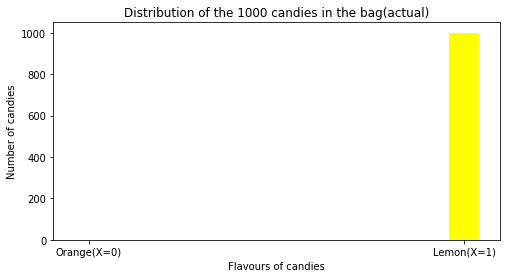
\includegraphics[scale=0.5]{Assignment1(1).png}
        \item 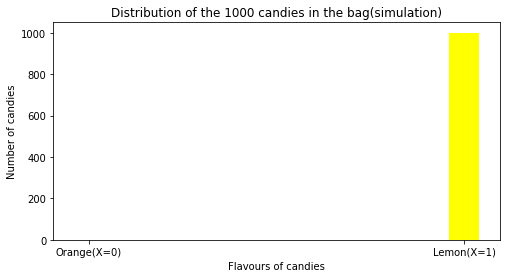
\includegraphics[scale=0.5]{Assignment1(2).png}
    \end{enumerate}
\end{enumerate}
\end{document}